% Generated by figmint | Journal: Science (AAAS) (science) | Spec version: 2025.1
% Guidelines: https://www.science.org/content/page/instructions-preparing-revised-manuscript
% Physical dimensions: 184.0 x 122.0 mm
\begin{figure}[t]
  \centering
  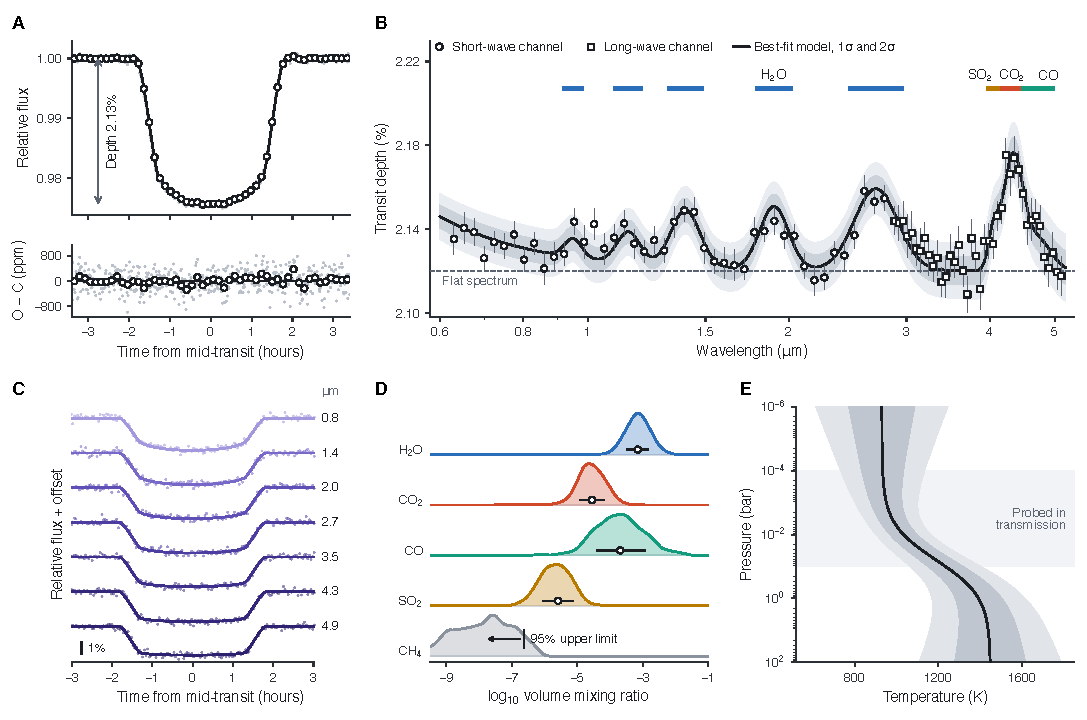
\includegraphics[width=184.0mm]{figure.pdf}
  \caption{Transmission spectrum of a warm giant exoplanet (synthetic data from a toy model, for illustration only). (A) White-light transit, with the best-fit model and binned points; residuals below. (B) Transit depth against wavelength from two detector channels, with the best-fit model and its 1σ and 2σ intervals; coloured bars mark absorption bands and the dashed line is a flat spectrum (no atmosphere). (C) Spectroscopic light curves, offset for clarity and labelled by wavelength. (D) Retrieved abundances; bars show the median and 68% interval. (E) Retrieved temperature-pressure profile with 1σ and 2σ intervals.}
  \label{fig:transmission-spectrum}
\end{figure}
